\documentclass[12pt]{article}
\usepackage{fullpage,enumitem,amsmath,amssymb,graphicx}

\title{Word Powering}
\author{Gene Li -- \texttt{gxli@princeton.edu}}

\begin{document}

\maketitle
\noindent

\section{Distributions of the Co-occurence Matrix}

\begin{enumerate}
\item Experimenting with co-occurence matrices generating by varying window sizes. Denote $M_k$ for $k= 1, 2, ...$ as the co-occurence matrix generated by using a window size of $k$.
\item Follow Arora's paper for the data preprocessing in order to ensure reproducible results.
\item How sparse is $M_k$ for different k? How does the sparsity grow?
\item How does the distribution of the co-occurence counts change? Which values get shrunk/grown when k is increased? i.e. is there a correlation $M_{2, ij}/M_{1, ij} \propto M_{1, ij}$?
\item Look at the graph powering $M_k^p$ for various k and p. How does the sparsity look now (should be densified). How do the distribution of values change?
\item Is it true that $M_1^2$ looks like $M_2$? Why or why not?
\end{enumerate}

\section{Quality of Word Embeddings}
\begin{enumerate}
\item Unweighted, vanilla SVD on (PMI) matrix. What is the performance for various k, various p?
\item What is the effect of truncation $\max(M_k, \kappa)$ operator?
\item Weighted SVD (PMI or SN). Now what?
\item Look at unweighted and weighted SVD on the graph that is powered. 
\item Observe the distribution of the vectors, and compare them.
\end{enumerate}

\section{Update 1}
\begin{itemize}
\item Looked at Arora's code found on SemanticVector. Since it uses C code to preprocess (which is adapted from GloVe, I opted to rewrite all the preprocessing in Python.
\item Downloaded and preprocessed wikipedia xml dump with text8 perl script to produce data/wikipedia\_raw. 
\item Using GloVe code to produce cooccurrence matrix. Script found in src/blah.sh. Produces the same cooccurrences as my old python code (which was too slow). Except for the (i,i) values - glove values are 2x my python script's values. This is probably not such an issue.
\item Converted the bin file of cooccurrence counts to a sparse matrix (.npz) for wikipedia.
\end{itemize}

\subsection{TODO}
\begin{itemize}
\item SVD on the PMI operator of the matrix, test that the resulting word vectors work on word similarity and analogy datasets. Unweighted matrix factorization provides a good baseline.
\item SVD on truncated PMI operator of the matrix, unweighted matrix factorization.
\item SVD on rand walk operator: $R = p(w|w')$. We can do something like $\hat{R} = \alpha R + (1-\alpha) R^2  $ Then apply the prior $p(w')$ to get an updated version of $p(w,w')$.
\item From here, decide where to go. Do we want to do weighted PMI? Do we want to use Arora's objective? Do we want to preprocess datasets with different window sizes?
\item Theoretically, how do we think about this as "smoothing" or regularization?
\end{itemize}

\subsection{Theory Thoughts}
It's not clear how truncation process (where we cap the maximum cooccurence at $X_{max}$) affects the spectral properties of the cooccurence matrix. One possible explanation is that it allows us to concentrate the "useless" words that don't give meaning ("and", "the", "so") etc. into the top eigenvector. In this way, we can effectively let the top eigenvector be "junk" syntax information, then the rest of the $d-1$ eigenvectors will be useful. If we don't truncate, maybe the useless words spread out over a few eigenvectors - say "the" appears in the 1st eigenvector, "and" appears in the 2nd eigenvector, etc. So we have more "junk" eigenvectors and thus, less useful eigendirections in our embedding.

I think this concept of "smoothing" is also useful. It appears in the sentence embedding paper and is a way for us to address the words that appear regardless of the discourse. Another way to think about the high degree nodes is to consider an SBM with $n$ vertices, split between two communities, where we have connectivity parameters $p, q$. Then, let us introduce "super-connected" nodes (some constant amount?) that connect equally to both communities with probability $r>p,q$. In this case, how do we detect the super-connected nodes? If we are able to detect, we can delete them from the graph and then do our community detection magic.

Is this a correct model for word embeddings? Does it make sense that some words connect strongly with other words, and have a relatively uniform distribution (connect equally). In our word embedding matrix, we can do some heuristics. We can delete them (say if the distribution is is roughly uniform and the overall probability $p(w)$ is large). Or we can apply some more continuous "smoothing" to account for this. I believe this is what the sentence embedding paper does.

One interesting fact: in the objective in RANDWALK, the optimization is scale invariant to the total \# of cooccurences. So we should be able to substitute empirical probabilities $p(w,w')$ in place of $X_{w,w'}$ and get the same resulting word vectors.

Maybe the correct definition for graph powering on word embeddings is on the random walk matrix $p(w|w').$ We can try to do some stuff like: square the random walk matrix. Then apply the prior $p(w')$ to get back to the joint probability $p(w,w')$. This basically smooths out the probabilities...? Intermediately, we can also try to smooth out the rows of the random walk matrix, as well as smooth out the prior $p(w')$. Is there an information-theoretic way to "smooth" out distributions? This could be interesting. The motivation here is that graph powering on the p(w,w') matrix is maybe not the right thing to do, because we just get everything routed on a walk to the "useless" words. 

An interesting thing: Taking the log is weird. If we take the log of an entry: $\sum_a p(w|a) p(a|w')$. It seems like we are approximately getting the MAX of $p(w|a)p(a|w')$ over a? (log-sum-exp approximation)This is related to what Enric suggest where we take the MAX along all paths. Maybe we should try to see if we can find a log expression of the conditional probability and build that into our objective. 

We should interpret graph powering, as well as truncation, NOT as producing a better estimate of the cooccurence counts in themselves. Instead, the correct (utilitst) viewpoint is to think of it as operations that allow us to construct $v_w$ to solve analogies/word similarity through matrix factorization, specifically for non "filler words". Can we accomplish something through manipulating the cooccurrence matrix through graph powering/ distribution smoothing in a similar way as the truncation effect does?

\section{Update 2}

\subsection{Thoughts}
\begin{itemize}
\item On text8, truncation seems to make word embeddings WORSE. 
\item Truncation reduces the tails of the unigram distribution (power law distribution) (green).
\item Truncation gives stronger concentration in the PMI values (in green).
\item For filler words, makes the values much more negative. 
\end{itemize}

\begin{figure}[h]
\centering
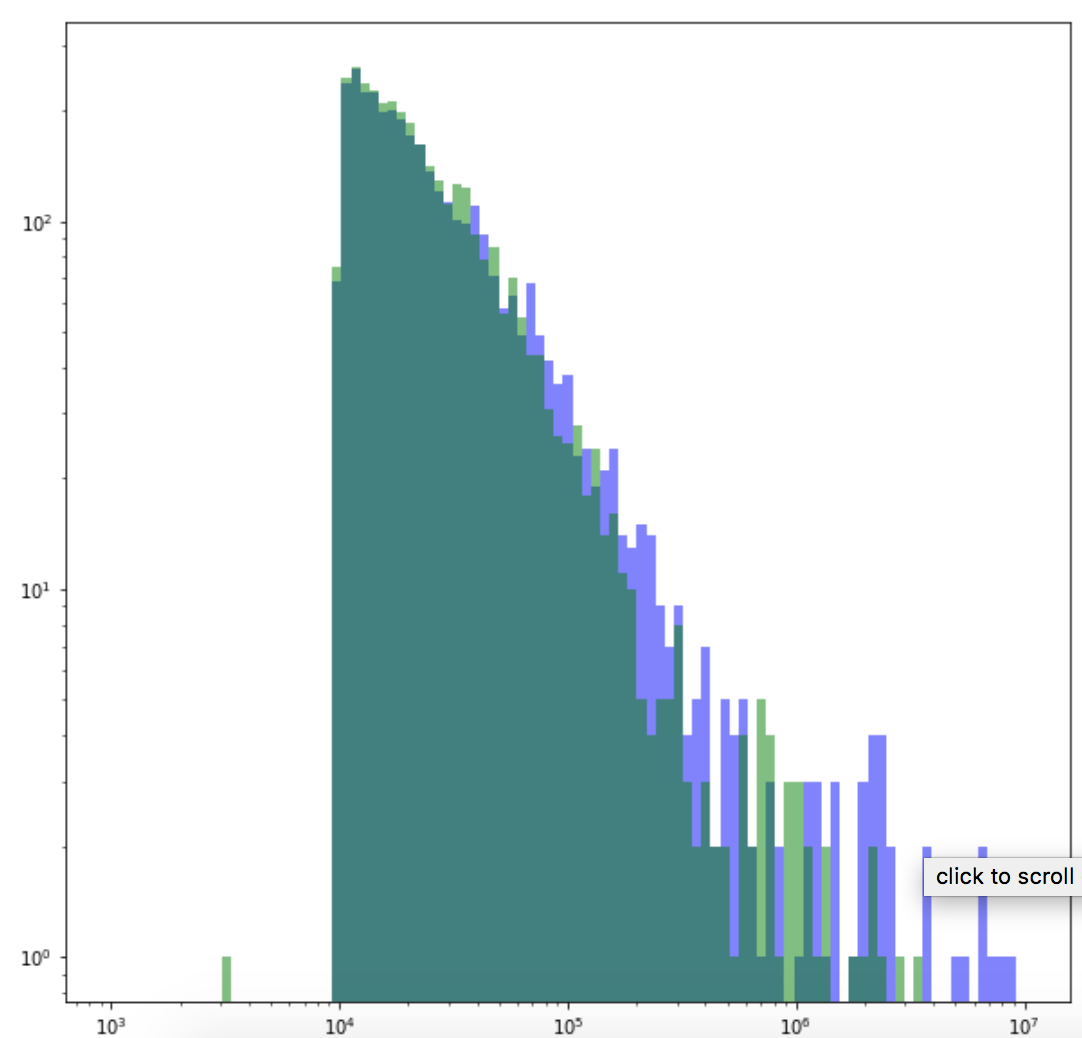
\includegraphics[width=10cm]{powerlawtext8.png}
\end{figure}

\begin{figure}[h]
\centering
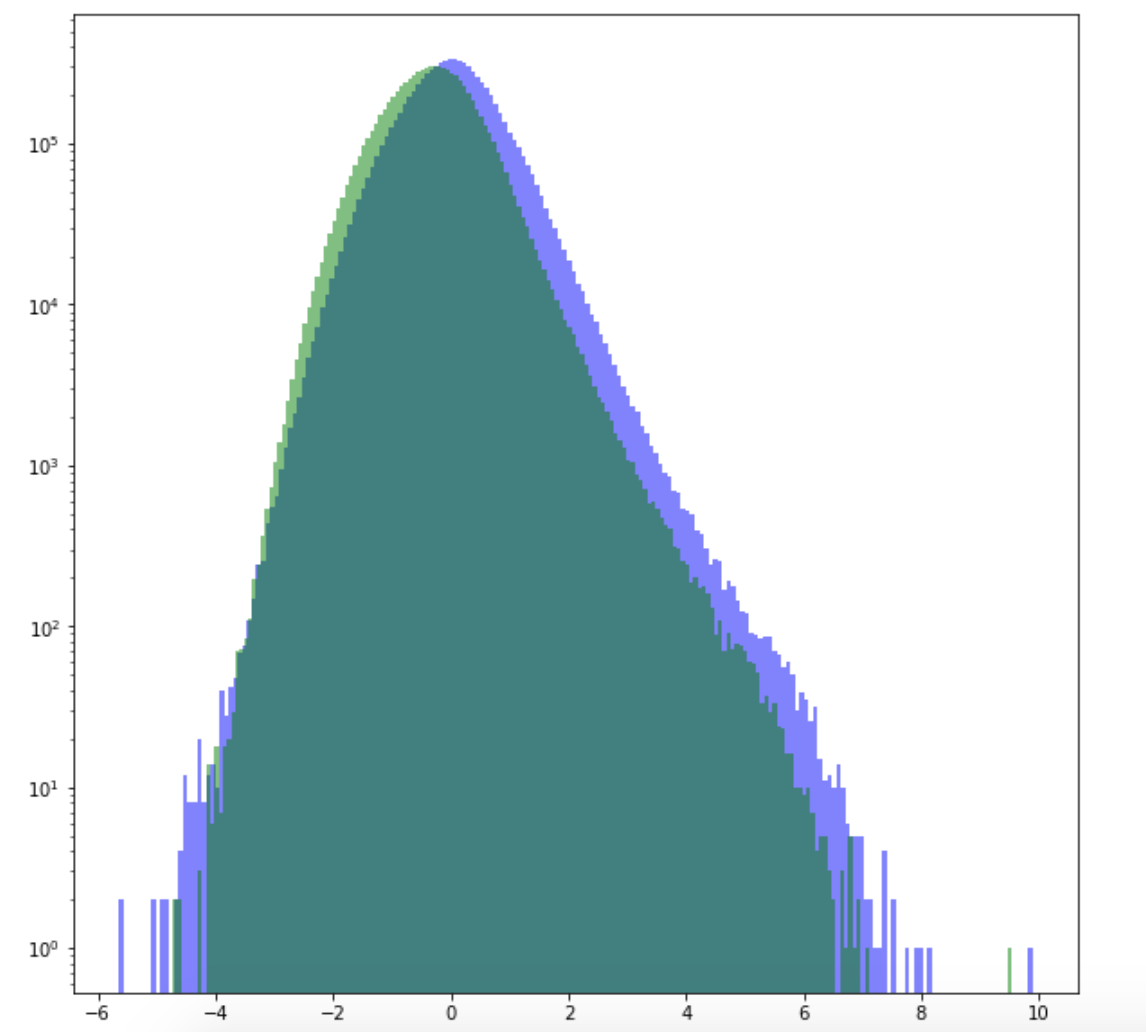
\includegraphics[width=10cm]{pmidisttext8.png}
\end{figure}

\section{Update 3}
\begin{itemize}
\item For co-counts matrix X, we can always normalize by sum of all values in X to get a co-occurrence empirical counts matrix. This does not affect vectors obtained by unweighted SVD on the PMI matrix.
\item Hence, let us think of X as $p(w,w')$. We can always factorize this as $p(w|w')*p(w')$. $p(w|w')$ is the random walk matrix if we interpret our words as a markov chain. 
\item Let us denote the matrix representing $p(w|w')$ as $R$ and the matrix $p(w') = D$, then $RD = X$. 
\item Then we can produce a new $\hat{R} = \alpha R + (1-\alpha) R^2$. Then we can write $\hat{X} = RD$.
\item When we run SVD on the PMI of $\hat{X}$, we get an improvement over $X$.
\end{itemize}

\begin{figure}[h]
\centering
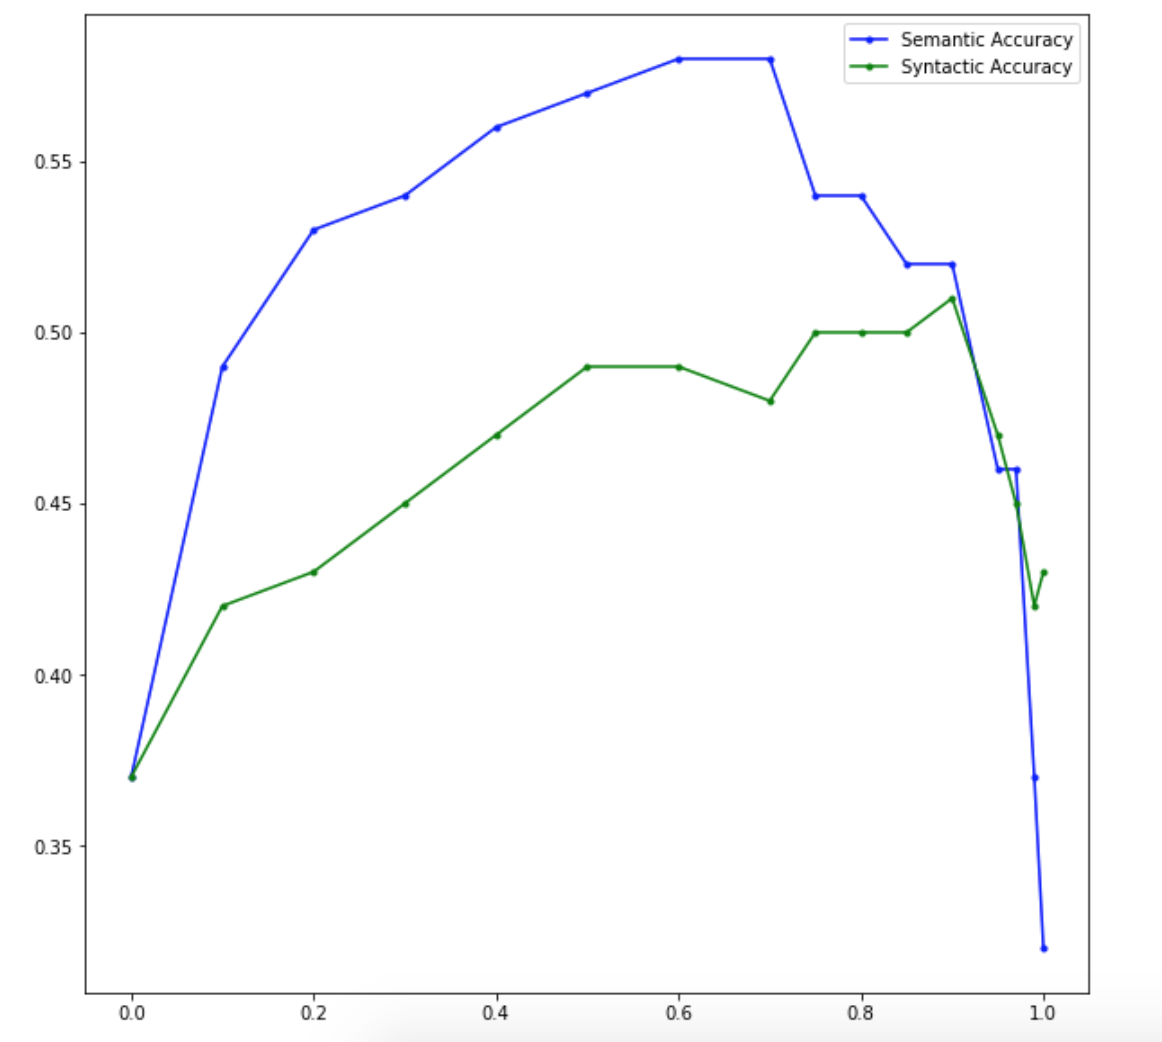
\includegraphics[width=10cm]{randwalkpower.png}
\end{figure}

\subsection{DONE}
\begin{itemize}
\item Also would be cool to look at a graph of how the values Aij are compared to ~Aij for those that are present in original data... as well as distribution of new values in ~Aij that were not seen before. 
\end{itemize}

\subsection{TODO}
\begin{itemize}
\item Run graph powering embeddings on Glove: 1) 50000 words, no powering 2) 50000 words, a=0.85 and square.
\item Think about squaring a submatrix - need to be smart about this. Apply some operator to X, then PMI. how do the two operations interact with each other? 
\item Is top spectral component concentrated around words with high unigram count? Is this useless for solving analogies?
\item graph sparsification?
\end{itemize}


\end{document}